\documentclass{beamer}
\usepackage[utf8x]{inputenc}
\usepackage{ucs}
\usepackage{amsmath}
\usepackage{amsfonts}
\usepackage{amssymb}
\usepackage{tikz}
\usetikzlibrary{arrows}
\usepackage{listings}
\usetheme{CambridgeUS}

\author{Cédric Guillot}
\institute{CPSC 565}
\title{Chess AI improvement through an evolutionary approach}
\date{April 9, 2013}

\begin{document}

\begin{frame}
\titlepage
\end{frame}

\begin{frame}
\begin{center}
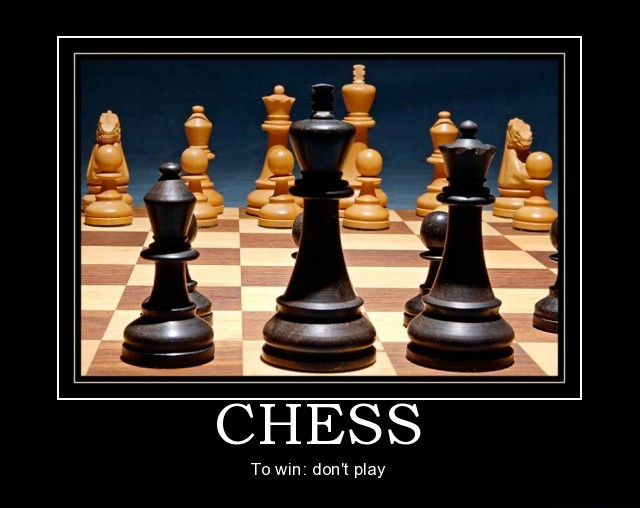
\includegraphics[scale=0.47]{images/to_win_dont_play.jpg}
\end{center}
\end{frame}

\begin{frame}
\tableofcontents
\end{frame}

\section{Introduction}
\begin{frame}
\frametitle{Chess AI history}
\begin{itemize}
\item 1951 - Alan Turing develops on paper the first program capable of playing a full game of chess
\item 1956 - John McCarthy invents the alpha-beta search algorithm
\item 1957 - First practical chess program, Alex Bernstein and a team of Russian programmers
\item 1981 - Cray Blitz becomes the first computer to gain a master rating (2200 ELO)
\item 1997 - Deep Blue wins a six-game match against Garry Kasparov
\item Today - Computers have reached 3250 ELO ratings
\end{itemize}
\end{frame}


\section{Implementation / Strategy}
\begin{frame}
\tableofcontents[currentsection]
\end{frame}

\begin{frame}
\subsection{Tools}
\frametitle{Tom Kerrigan's Simple Chess Program (TSCP)}
\begin{itemize}
\item Chess engine used for playing all the games
\item Written in 1997
\item Negamax algorithm for the AI
\end{itemize}
\end{frame}

\begin{frame}
\frametitle{GUI: GNU Xboard}
\begin{center}
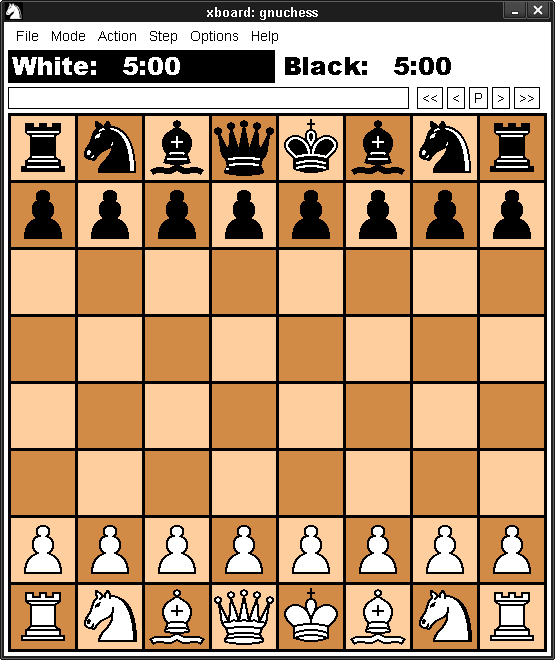
\includegraphics[scale=0.3]{images/xboard_view.png}
\end{center}
\end{frame}

\begin{frame}
\subsection{Architecture}
\frametitle{Architecture}
\begin{center}
\begin{figure}
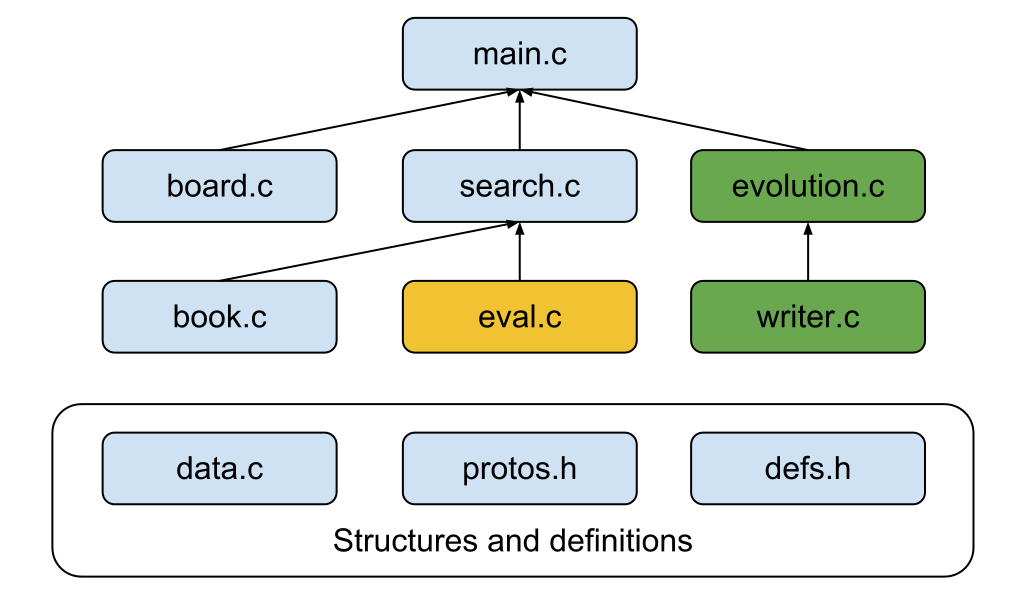
\includegraphics[scale=0.3]{images/Chess_AI_Architecture.png}
\caption{TSCP and evolution algorithm plugin architecture}
\end{figure}
\end{center}
\end{frame}

\begin{frame}
\subsection{Board evaluation / parameters evaluation}
\frametitle{Board evaluation / parameters evaluation}
\begin{itemize}
\item Board evaluated at each move during the game, using the pieces values
\item Individuals of the same generation compete against each other
\begin{itemize}
\item $\frac{n(n-1)}{2}$ games per generation
\item one game as white, one as black
\end{itemize}
\item Point system: 0 for loss, 3 for win, 1 for stalemate or draw
\end{itemize}
\end{frame}

\section{Results}
\begin{frame}
\tableofcontents[currentsection]
\end{frame}

\begin{frame}
\subsection{Set-up}
\frametitle{Set-up}
\begin{itemize}
\item Search depth: n = 1
\item One day and a half running on a standard laptop
\item Optimized parameters: pawn(100), knight(300), bishop(300), rook(500) and queen(900) values
\item Evolution strategy parameters: $\mu = \frac{1}{2} \lambda = 4$
\item Static strategy parameters: RAND(-15, 15)
\end{itemize}
\end{frame}

\begin{frame}
\subsection{Evolved AI}
\frametitle{Evolved AI}
\begin{itemize}
\item Original AI against human
\item Evolved AI
\end{itemize}
\end{frame}

\begin{frame}
\begin{center}
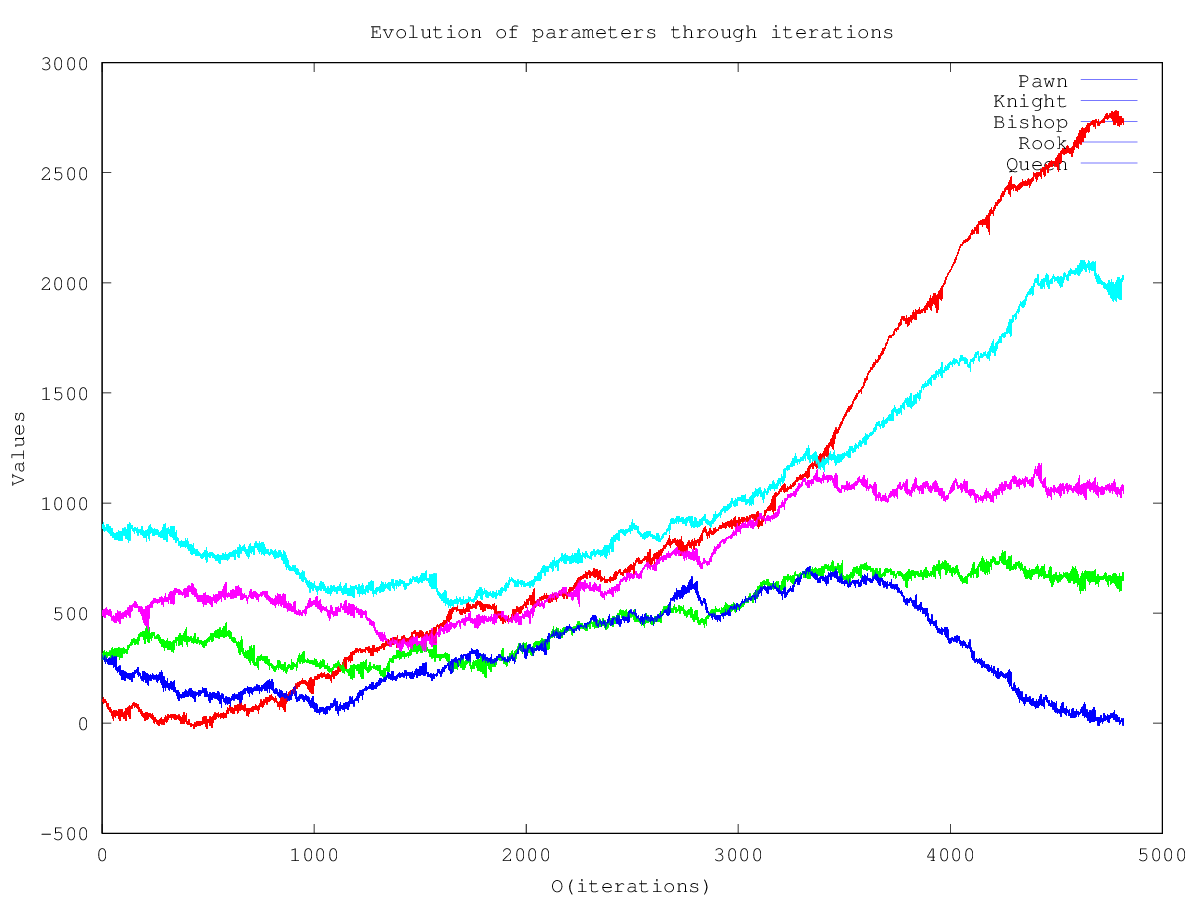
\includegraphics[scale=0.5]{../results/history_individuals_1.png}
\end{center}
\end{frame}

\section{Future work}
\begin{frame}
\tableofcontents[currentsection]
\end{frame}

\begin{frame}
\frametitle{Future work}
\begin{itemize}
\item Stabilize the algorithm
\begin{itemize}
\item Boundaries for values
\end{itemize}
\item Evolving strategy parameters
\end{itemize}
\end{frame}

\begin{frame}
\frametitle{References}
\begin{itemize}
\item Hallam Nasreddine, Hendra Suhanto Poh and Graham Kendall : Using an Evolutionary Algorithm for the Tuning of a Chess Evaluation Function Based on a Dynamic Boundary Strategy\\
http://red.cs.nott.ac.uk/~gxk/papers/ieeecis2006.pdf

\item DAVID B. FOGEL, FELLOW, IEEE, TIMOTHY J. HAYS, SARAH L. HAHN, AND JAMES QUON : A Self-Learning Evolutionary Chess Program\\
http://ieeexplore.ieee.org/stamp/stamp.jsp?tp=\&arnumber=1360168

\item Graham Kendall, Glenn Whitwell : An Evolutionary Approach for the Tuning of a
Chess Evaluation Function using Population Dynamics\\
http://ieeexplore.ieee.org/stamp/stamp.jsp?tp=\&arnumber=934299
\end{itemize}
\end{frame}

\begin{frame}
\frametitle{Questions}
\begin{center}
\begin{Huge}
Any questions or suggestions?
\end{Huge}
\end{center}
\end{frame}

\end{document}
